\documentclass[10pt,a4paper]{article}
\usepackage[T1]{fontenc}
\usepackage[utf8]{inputenc}
\usepackage{lmodern}
\usepackage[margin=0.55in]{geometry}
\usepackage{xcolor}
\usepackage{tikz}
\usepackage{tabularx}
\usepackage{booktabs}
\usepackage{array}
\usepackage{enumitem}
\usepackage{hyperref}
\usetikzlibrary{arrows.meta,positioning,fit,backgrounds,calc,shapes.multipart}

\definecolor{brandgreen}{HTML}{14A44D}
\definecolor{branddark}{HTML}{0F172A}
\definecolor{brandslate}{HTML}{334155}
\definecolor{brandblue}{HTML}{2563EB}
\definecolor{brandamber}{HTML}{D97706}
\definecolor{brandred}{HTML}{DC2626}
\definecolor{brandviolet}{HTML}{7C3AED}
\definecolor{boxfill}{HTML}{F8FAFC}
\definecolor{boxline}{HTML}{CBD5E1}
\definecolor{softgreen}{HTML}{DCFCE7}
\definecolor{softblue}{HTML}{DBEAFE}
\definecolor{softamber}{HTML}{FEF3C7}
\definecolor{softred}{HTML}{FEE2E2}
\definecolor{softviolet}{HTML}{EDE9FE}

\hypersetup{
  colorlinks=true,
  linkcolor=brandblue,
  urlcolor=brandblue
}

\pagestyle{plain}
\setlength{\parindent}{0pt}
\setlength{\parskip}{4pt}
\renewcommand{\arraystretch}{1.15}

\tikzset{
  archbox/.style={
    rounded corners=5pt,
    draw=boxline,
    fill=boxfill,
    line width=0.8pt,
    align=center,
    font=\footnotesize,
    minimum height=0.9cm,
    inner sep=6pt
  },
  titlebox/.style={
    archbox,
    fill=branddark!4,
    draw=brandslate,
    font=\bfseries\footnotesize
  },
  greenbox/.style={archbox, fill=softgreen},
  bluebox/.style={archbox, fill=softblue},
  amberbox/.style={archbox, fill=softamber},
  redbox/.style={archbox, fill=softred},
  violetbox/.style={archbox, fill=softviolet},
  arrow/.style={-{Latex[length=2.2mm,width=1.6mm]}, line width=0.8pt, draw=brandslate},
  dashedarrow/.style={arrow, dashed},
  group/.style={rounded corners=7pt, draw=brandslate!55, dashed, inner sep=8pt}
}

\begin{document}

{\LARGE\bfseries AgriAdvisor Production Architecture}\\[-1mm]
{\small Multilingual mobile and web agricultural advisory platform with resilient orchestration, fallback reasoning, translation, and voice interfaces}

\vspace{2mm}
\hrule
\vspace{3mm}

\textbf{Architecture objective.}
This design documents the current production-oriented architecture of the AgriAdvisor application in the repository. It is intentionally more detailed than a prototype diagram: it captures the runtime layers, state ownership, multilingual processing path, fallback behavior, data providers, and voice interfaces that together make the system usable on both mobile and web.

\begin{center}
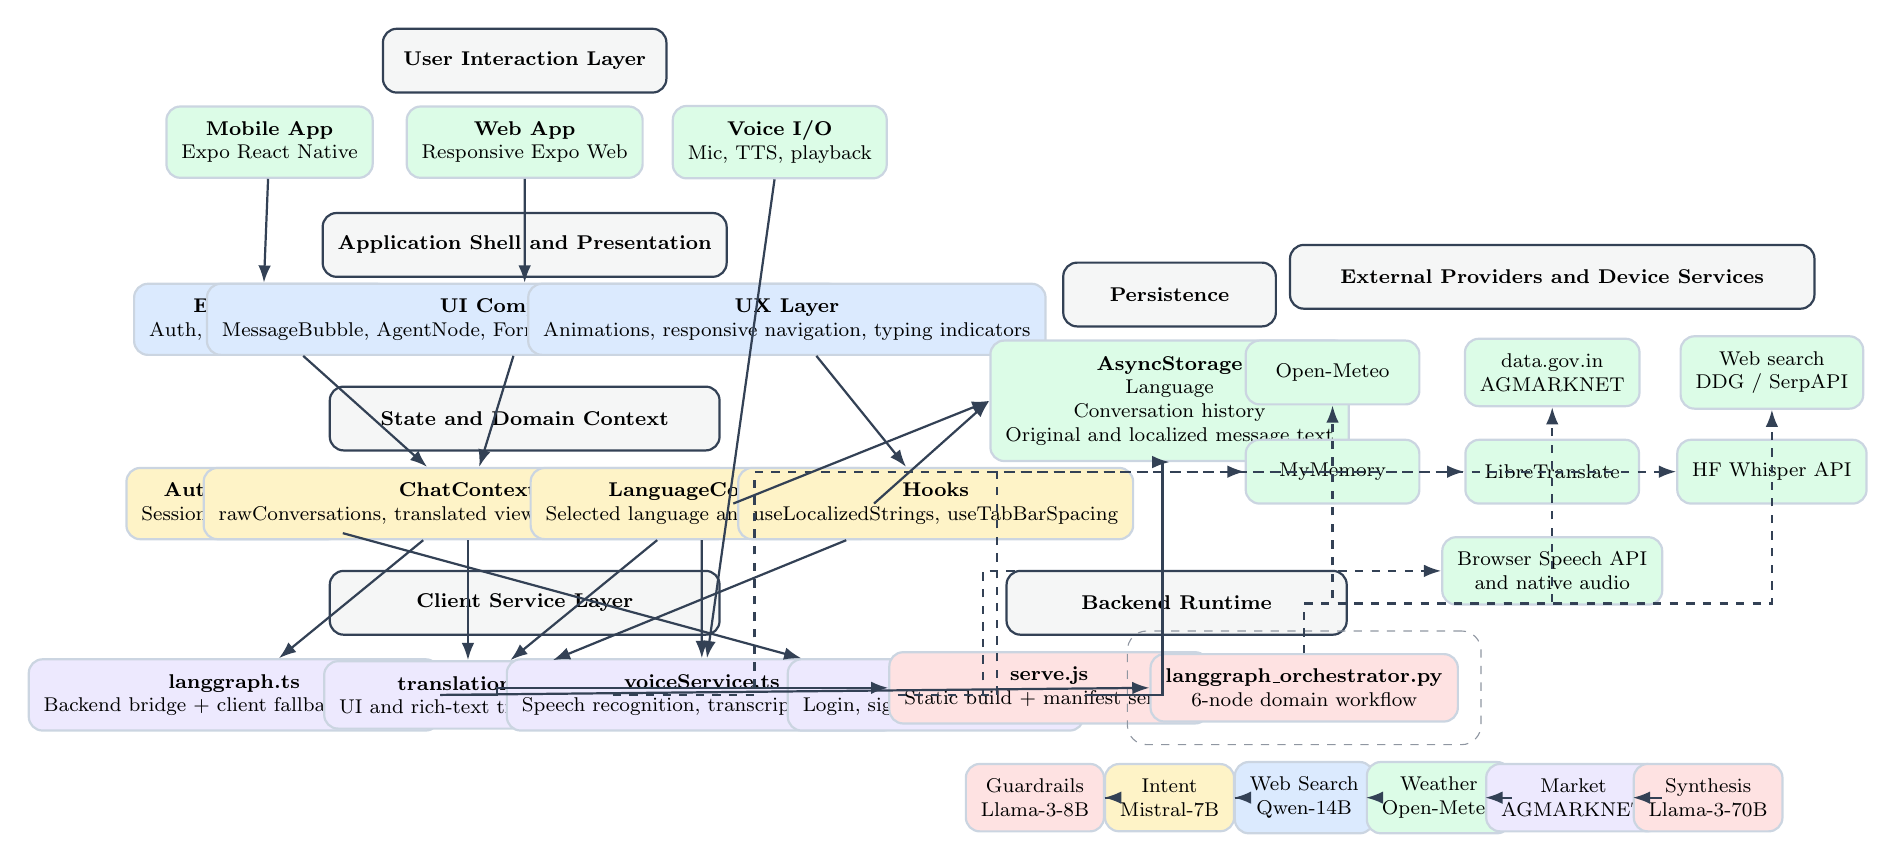
\begin{tikzpicture}[x=1cm,y=1cm, font=\footnotesize, scale=0.9, transform shape]
  % User layer
  \node[titlebox, minimum width=4.0cm] (users) at (5.8,10.6) {User Interaction Layer};
  \node[greenbox, minimum width=2.6cm] (mobile) at (2.2,9.45) {\textbf{Mobile App}\\Expo React Native};
  \node[greenbox, minimum width=2.6cm] (web) at (5.8,9.45) {\textbf{Web App}\\Responsive Expo Web};
  \node[greenbox, minimum width=2.6cm] (voiceui) at (9.4,9.45) {\textbf{Voice I/O}\\Mic, TTS, playback};

  % App shell
  \node[titlebox, minimum width=5.5cm] (shelltitle) at (5.8,8.0) {Application Shell and Presentation};
  \node[bluebox, minimum width=3.2cm] (router) at (2.1,6.95) {\textbf{Expo Router}\\Auth, Tabs, Chat Detail};
  \node[bluebox, minimum width=3.2cm] (ui) at (5.8,6.95) {\textbf{UI Components}\\MessageBubble, AgentNode, FormattedAIContent, AppBackdrop};
  \node[bluebox, minimum width=3.2cm] (ux) at (9.5,6.95) {\textbf{UX Layer}\\Animations, responsive navigation, typing indicators};

  % State layer
  \node[titlebox, minimum width=5.5cm] (statetitle) at (5.8,5.55) {State and Domain Context};
  \node[amberbox, minimum width=2.7cm] (authctx) at (1.7,4.35) {\textbf{AuthContext}\\Session and identity};
  \node[amberbox, minimum width=2.7cm] (chatctx) at (5.0,4.35) {\textbf{ChatContext}\\rawConversations, translated view, message metadata};
  \node[amberbox, minimum width=2.7cm] (langctx) at (8.3,4.35) {\textbf{LanguageContext}\\Selected language and persistence};
  \node[amberbox, minimum width=2.7cm] (hooks) at (11.6,4.35) {\textbf{Hooks}\\useLocalizedStrings, useTabBarSpacing};

  % Services
  \node[titlebox, minimum width=5.5cm] (servicetitle) at (5.8,2.95) {Client Service Layer};
  \node[violetbox, minimum width=2.9cm] (langgraph) at (1.7,1.65) {\textbf{langgraph.ts}\\Backend bridge + client fallback pipeline};
  \node[violetbox, minimum width=2.9cm] (translation) at (5.0,1.65) {\textbf{translation.ts}\\UI and rich-text translation};
  \node[violetbox, minimum width=2.9cm] (voice) at (8.3,1.65) {\textbf{voiceService.ts}\\Speech recognition, transcription, TTS};
  \node[violetbox, minimum width=2.9cm] (authsvc) at (11.6,1.65) {\textbf{auth.ts}\\Login, signup, password flow};

  % Persistence
  \node[titlebox, minimum width=3.0cm] (persisttitle) at (14.9,7.3) {Persistence};
  \node[greenbox, minimum width=3.0cm, minimum height=1.7cm] (store) at (14.9,5.8) {\textbf{AsyncStorage}\\Language\\Conversation history\\Original and localized message text};

  % Backend group
  \node[titlebox, minimum width=4.8cm] (backendtitle) at (15.0,2.95) {Backend Runtime};
  \node[redbox, minimum width=3.0cm] (nodeserver) at (13.2,1.75) {\textbf{serve.js}\\Static build + manifest serving};
  \node[redbox, minimum width=3.3cm] (orchestrator) at (16.8,1.75) {\textbf{langgraph\_orchestrator.py}\\6-node domain workflow};

  % Pipeline group
  \node[group, fit=(orchestrator)] (pipefit) {};
  \node[archbox, minimum width=1.75cm, fill=softred] (g1) at (13.0,0.2) {Guardrails\\Llama-3-8B};
  \node[archbox, minimum width=1.75cm, fill=softamber] (g2) at (14.9,0.2) {Intent\\Mistral-7B};
  \node[archbox, minimum width=1.75cm, fill=softblue] (g3) at (16.8,0.2) {Web Search\\Qwen-14B};
  \node[archbox, minimum width=1.75cm, fill=softgreen] (g4) at (18.7,0.2) {Weather\\Open-Meteo};
  \node[archbox, minimum width=1.75cm, fill=softviolet] (g5) at (20.6,0.2) {Market\\AGMARKNET};
  \node[archbox, minimum width=1.75cm, fill=softred] (g6) at (22.5,0.2) {Synthesis\\Llama-3-70B};

  % External services
  \node[titlebox, minimum width=7.4cm] (externaltitle) at (20.3,7.55) {External Providers and Device Services};
  \node[greenbox, minimum width=2.45cm] (weatherapi) at (17.2,6.2) {Open-Meteo};
  \node[greenbox, minimum width=2.45cm] (marketapi) at (20.3,6.2) {data.gov.in\\AGMARKNET};
  \node[greenbox, minimum width=2.45cm] (searchapi) at (23.4,6.2) {Web search\\DDG / SerpAPI};
  \node[greenbox, minimum width=2.45cm] (mymemory) at (17.2,4.8) {MyMemory};
  \node[greenbox, minimum width=2.45cm] (libre) at (20.3,4.8) {LibreTranslate};
  \node[greenbox, minimum width=2.45cm] (hf) at (23.4,4.8) {HF Whisper API};
  \node[greenbox, minimum width=2.45cm] (speechdev) at (20.3,3.4) {Browser Speech API\\and native audio};

  % arrows
  \draw[arrow] (mobile) -- (router);
  \draw[arrow] (web) -- (ui);
  \draw[arrow] (voiceui) -- (voice);
  \draw[arrow] (router) -- (chatctx);
  \draw[arrow] (ui) -- (chatctx);
  \draw[arrow] (ux) -- (hooks);
  \draw[arrow] (authctx) -- (authsvc);
  \draw[arrow] (chatctx) -- (langgraph);
  \draw[arrow] (chatctx) -- (translation);
  \draw[arrow] (langctx) -- (translation);
  \draw[arrow] (langctx) -- (voice);
  \draw[arrow] (hooks) -- (translation);
  \draw[arrow] (chatctx.east) -- (store.west);
  \draw[arrow] (langctx.east) -- (store.west);
  \draw[arrow] (authsvc.east) -- ++(1.1,0) |- (store.south);
  \draw[arrow] (langgraph.east) -- (orchestrator.west);
  \draw[arrow] (langgraph.east) -- ++(0.8,0) |- (nodeserver.west);
  \draw[dashedarrow] (translation.east) -- ++(2.0,0) |- (mymemory.west);
  \draw[dashedarrow] (translation.east) -- ++(2.0,0) |- (libre.west);
  \draw[dashedarrow] (voice.east) -- ++(1.4,0) |- (hf.west);
  \draw[dashedarrow] (voice.east) -- ++(1.2,0) |- (speechdev.west);
  \draw[dashedarrow] (orchestrator.north) -- ++(0,0.7) -| (weatherapi.south);
  \draw[dashedarrow] (orchestrator.north) -- ++(0,0.7) -| (marketapi.south);
  \draw[dashedarrow] (orchestrator.north) -- ++(0,0.7) -| (searchapi.south);

  \draw[arrow] (g1) -- (g2);
  \draw[arrow] (g2) -- (g3);
  \draw[arrow] (g3) -- (g4);
  \draw[arrow] (g4) -- (g5);
  \draw[arrow] (g5) -- (g6);
\end{tikzpicture}
\end{center}

\textbf{Design notes.}
\begin{itemize}[leftmargin=5mm,itemsep=1mm,topsep=1mm]
  \item \textbf{Single app surface, dual runtime:} the same Expo codebase serves mobile and web, while the navigation shell adapts to the target form factor.
  \item \textbf{Language-aware state model:} the chat layer stores both localized content and a stable base version so UI language changes can re-render conversations instead of locking them to the previous language.
  \item \textbf{Operational resilience:} if the backend pipeline is unavailable, the client still produces structured agricultural advice using local intent detection, live API fetches, and curated fallback builders.
  \item \textbf{Voice integration is not cosmetic:} voice input, transcription, speech playback, and multilingual text normalization are treated as first-class interaction channels.
\end{itemize}

\clearpage

{\Large\bfseries Runtime Request and Response Lifecycle}

\vspace{1mm}
\textbf{Execution model.}
Every advisory request follows a multilingual normalization path first, then chooses the highest-fidelity available processing route. The architecture is designed so the user still receives a valid response when any one subsystem becomes unavailable.

\begin{center}
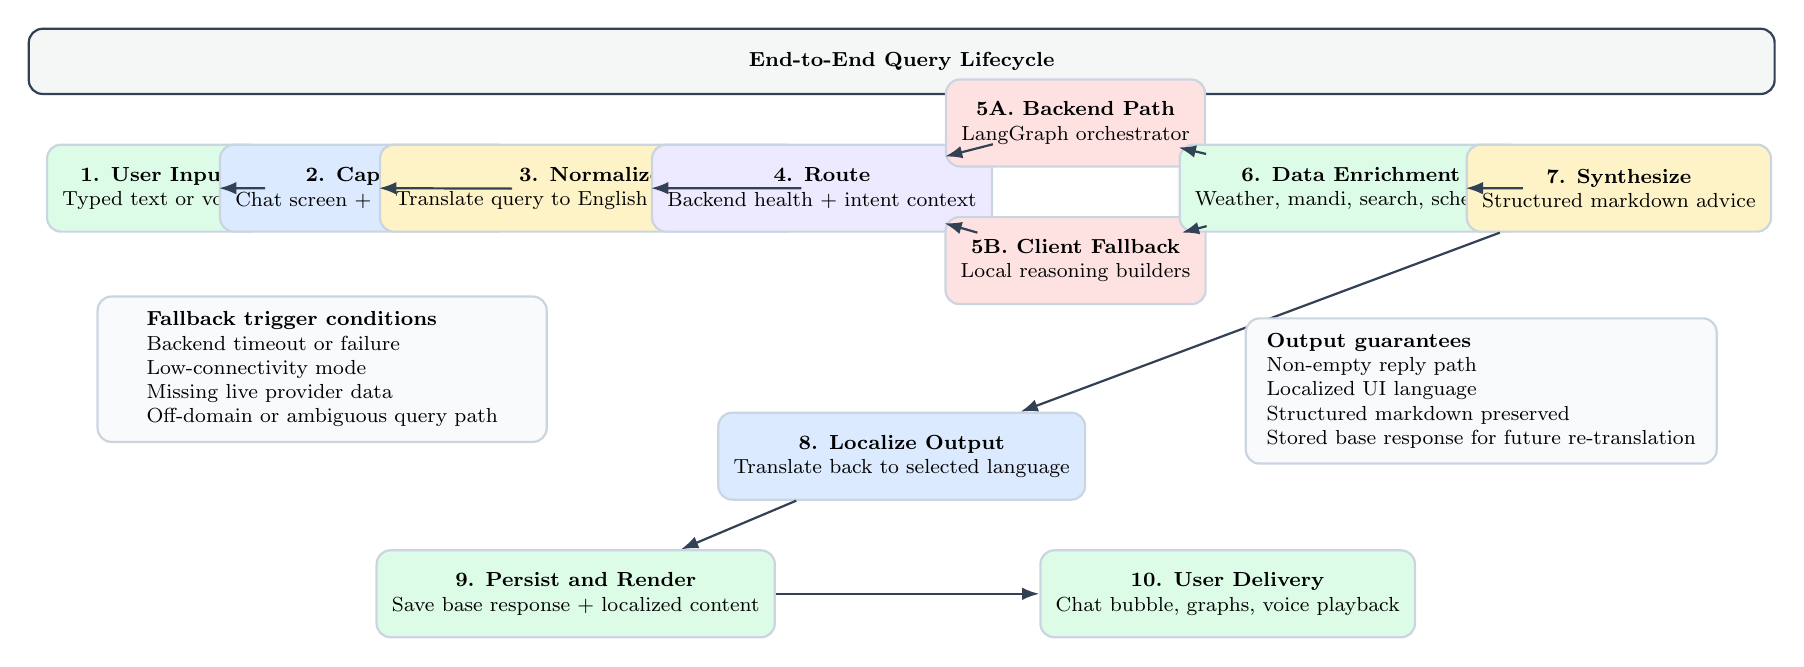
\begin{tikzpicture}[x=1cm,y=1cm, font=\footnotesize, scale=0.92, transform shape]
  \node[titlebox, minimum width=24.1cm] (lifetitle) at (12.0,8.65) {End-to-End Query Lifecycle};

  \node[greenbox, minimum width=2.4cm, minimum height=1.2cm] (s1) at (1.7,6.9) {\textbf{1. User Input}\\Typed text or voice};
  \node[bluebox, minimum width=2.4cm, minimum height=1.2cm] (s2) at (4.6,6.9) {\textbf{2. Capture}\\Chat screen + voice service};
  \node[amberbox, minimum width=2.5cm, minimum height=1.2cm] (s3) at (7.7,6.9) {\textbf{3. Normalize}\\Translate query to English for processing};
  \node[violetbox, minimum width=2.5cm, minimum height=1.2cm] (s4) at (10.9,6.9) {\textbf{4. Route}\\Backend health + intent context};
  \node[redbox, minimum width=2.8cm, minimum height=1.2cm] (s5a) at (14.4,7.8) {\textbf{5A. Backend Path}\\LangGraph orchestrator};
  \node[redbox, minimum width=2.8cm, minimum height=1.2cm] (s5b) at (14.4,5.9) {\textbf{5B. Client Fallback}\\Local reasoning builders};
  \node[greenbox, minimum width=3.0cm, minimum height=1.2cm] (s6) at (18.2,6.9) {\textbf{6. Data Enrichment}\\Weather, mandi, search, schemes};
  \node[amberbox, minimum width=2.8cm, minimum height=1.2cm] (s7) at (21.9,6.9) {\textbf{7. Synthesize}\\Structured markdown advice};
  \node[bluebox, minimum width=2.8cm, minimum height=1.2cm] (s8) at (12.0,3.2) {\textbf{8. Localize Output}\\Translate back to selected language};
  \node[greenbox, minimum width=3.4cm, minimum height=1.2cm] (s9) at (7.5,1.3) {\textbf{9. Persist and Render}\\Save base response + localized content};
  \node[greenbox, minimum width=3.4cm, minimum height=1.2cm] (s10) at (16.5,1.3) {\textbf{10. User Delivery}\\Chat bubble, graphs, voice playback};

  \draw[arrow] (s1) -- (s2);
  \draw[arrow] (s2) -- (s3);
  \draw[arrow] (s3) -- (s4);
  \draw[arrow] (s4) -- (s5a);
  \draw[arrow] (s4) -- (s5b);
  \draw[arrow] (s5a) -- (s6);
  \draw[arrow] (s5b) -- (s6);
  \draw[arrow] (s6) -- (s7);
  \draw[arrow] (s7) -- (s8);
  \draw[arrow] (s8) -- (s9);
  \draw[arrow] (s9) -- (s10);

  \node[archbox, minimum width=6.2cm, align=left] (notea) at (4.0,4.4) {
    \textbf{Fallback trigger conditions}\\
    Backend timeout or failure\\
    Low-connectivity mode\\
    Missing live provider data\\
    Off-domain or ambiguous query path
  };

  \node[archbox, minimum width=6.5cm, align=left] (noteb) at (20.0,4.1) {
    \textbf{Output guarantees}\\
    Non-empty reply path\\
    Localized UI language\\
    Structured markdown preserved\\
    Stored base response for future re-translation
  };
\end{tikzpicture}
\end{center}

\textbf{Component responsibility summary.}

\begin{tabularx}{\textwidth}{>{\raggedright\arraybackslash}p{2.7cm} >{\raggedright\arraybackslash}X >{\raggedright\arraybackslash}p{4.6cm}}
\toprule
\textbf{Layer} & \textbf{Primary responsibility} & \textbf{Key implementation artifacts} \\
\midrule
Presentation & Responsive mobile/web UI, chat rendering, graph/table formatting, voice controls, animated navigation & \texttt{app/(tabs)/*}, \texttt{app/chat/[id].tsx}, \texttt{components/MessageBubble.tsx}, \texttt{components/FormattedAIContent.tsx} \\
State management & Authentication state, language selection, conversation storage, message mutation, translated conversation view & \texttt{context/AuthContext.tsx}, \texttt{context/LanguageContext.tsx}, \texttt{context/ChatContext.tsx} \\
Client intelligence & Query normalization, backend routing, multilingual translation, speech recognition, transcription, speech playback & \texttt{services/langgraph.ts}, \texttt{services/translation.ts}, \texttt{services/voiceService.ts} \\
Backend orchestration & Domain-safe reasoning workflow with auditable node execution and model specialization & \texttt{backend/langgraph\_orchestrator.py}, \texttt{server/serve.js} \\
External dependencies & Weather, market data, search, translation, Whisper transcription, browser speech runtime & Open-Meteo, AGMARKNET data.gov.in, MyMemory, LibreTranslate, Hugging Face, device speech APIs \\
\bottomrule
\end{tabularx}

\vspace{2mm}
\textbf{Why this is stronger than a prototype.}
\begin{itemize}[leftmargin=5mm,itemsep=1mm,topsep=1mm]
  \item The design explicitly separates \textbf{base response storage} from \textbf{localized rendering}, which is required for language switching across old and new chats.
  \item It includes a \textbf{degraded-mode operating path} rather than assuming the orchestrator is always available.
  \item It models \textbf{voice, translation, and persistence} as architectural subsystems, not UI add-ons.
  \item It documents the \textbf{true external contracts} the application depends on, which is necessary for deployment, testing, and failure analysis.
\end{itemize}

\vfill
{\small Recommended build command: \texttt{pdflatex agriadvisor-architecture.tex}}

\end{document}
